\documentclass{standalone}
\usepackage{pgfplots}
\begin{document}
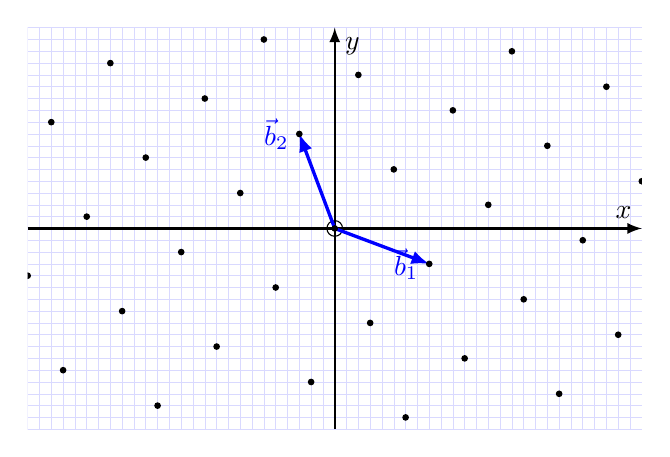
\begin{tikzpicture}[scale=.15]
  \clip(-26,-17)  rectangle (26,17);
   \coordinate (Origin) at (0,0); 
   \coordinate (Bone) at (8,-3);
   \coordinate (Btwo) at (-3,8);
     \draw[style=help lines,color=blue!15] (-26,-20) grid[step=1cm] (26,20);
%     \draw[style=help lines,thin,dotted] (-26,-20) grid[step=1cm] (26,20);
   \draw[thick,-latex] (-26,0) -- (26,0) node [above left] {$x$};
  \draw[thick,-latex] (0,-17) -- (0,17) node [below right] {$y$};
  \node[draw,circle,inner sep=2pt] at (0,0) {};     
  \draw [very thick,-latex,blue] (Origin)    -- (Bone) node [left] {$\vec b_1$};
     \draw [very thick,-latex,blue] (Origin)   -- (Btwo) node [left] {$\vec b_2$};
  \foreach \y in {-5,-4,...,5}{%Two indices running over each 
      \foreach \x in {-5,-4,...,5}{% node on the grid we have drawn
    \node[draw,circle,inner sep=.7pt,fill] at (8*\x-3*\y,-3*\x+8*\y) {};
    }
    }
 \end{tikzpicture}
 \end{document}